\chapter{How congestion shapes cities}

Empirical evidence suggest that most urban systems experience a
transition from a monocentric to a polycentric organisation as they
grow and expand. We propose here a stochastic, out-of-equilibrium model of the
city which explains the appearance of subcenters as an effect of
traffic congestion. We show that congestion triggers the unstability
of the monocentric regime, and that the number of subcenters and the
total commuting distance within a city scale sublinearly with its
population, predictions which are in agreement with data gathered for
around 9000 US cities between 1994 and 2010.\\


As cities grow, they evolve from a monocentric organisation where all
the activities are concentrated in the same geographical area
--usually the central business district-- to a more distributed,
polycentric organisation~\cite{Kemper:1974,Odland:1978,Mills:1972,Griffith_PG:1981,Dokmeci:1994,McMillen:2003,Pereira:2013,Roth:2011}.  However, these approaches fail
at giving a satisfactory quantitative
account~\cite{Bouchaud:2008,Batty:2008} of the polycentric transition
of cities. First, they describe a city as being in an equilibrium
characterised by static spatial distributions of households and business
firms. However, the equilibrium assumption is unsupported as cities
are out-of-equilibrium systems and their
dynamics is of particular interest for practical
applications~\cite{Batty:2008}. Second, these models integrate so many
interactions and variables that it is difficult to understand the
hierarchy of processes governing the evolution of cities, which ones are fundamental and which ones a irrelevant. Yet, traffic congestion is not
explicitly taken into account in the existing models, despite being
mentioned in the economics literature as a possible reason for the
polycentric transition~\cite{McMillen:2003}. Lastly, the models do
not make any quantitative prediction and are therefore unsupported by
data.\\ 
We present in this Letter a stochastic, out-of-equilibrium model of the
city which relies on the assumption that the polycentric structure of
large cities might find its origin in congestion, irrespective of the
particular local economic details. We are able to reproduce many
stylized facts, and --most importantly-- to derive a general relation
between the number of activity centers of a city and its
population. Finally, we verify this relation against the employment
data from around 9000 cities in the US between 1994 and 2010.

%\section{The model}

Following recent interdisciplinary efforts to construct a quantitative
description of cities and their
evolution~\cite{Makse:1995,Zanette:1997,Marsili:1998a,Marsili:1998b,Batty:book2005,Bettencourt:2007,Batty:2008},
we deliberately omit certain details and focus instead on basic
processes. We thereby aim at building a minimal model which captures
the complexity of the system and is able to account for --qualitative as well as quantitive-- stylized
facts. The model we propose is by essence dynamical and describes the
evolution of cities' organisation as their population increases. We
focus on car congestion --mainly due to journey-to-work commutes --
and its effect on the job location choice for individuals.

\section{Fujita and Ogawa}
\label{sec:fujita_and_ogawa}

In line with the tradition of economic geography~\cite{Fujita:2001}, the model
of Fujita and Ogawa~\cite{Fujita:1982} is based on the concept of agglomeration
economies---to explain why economical activities tend to group---and the spatial
distribution of wages and rents across the urban space. They consider that
cities are constituted of two kinds of actors: the firms, who tend to
concentrate to maximise their production, and the households, who try to
minimise their rent and commuting cost. In the following, I will present the
model with somewhat simplified notations\graffito{In particular, I dropped the
explicit mention of land consumption, and labour force since they are `assumed
out' of the model.} focusing on the hypotheses and the results.\\ 

The model is \emph{static}, in the sense that the number of firms and
individuals are fixed. It is an \emph{equilibrium} model, considering the the
city is the realisation of a general optimum. The original model is also
\emph{one-dimensional}, although the hypothesis of one-dimensionality is not
fundamental, and only necessary to make the calculations easier. Because I will
not try to solve the model, I will write equations in the 2D case.

\subsection{Households} 
\label{sub:households}

Fujita and Ogawa assume that there is a fixed number $N$ of households in the
city. The households are considered identical, in the sense that they all have
the same utility function and the same budget constraint. The utility function
of each household is given by the function $U = U(Z)$ where $Z$ is the surplus
of money that is left after budgetary constraints (expressed in monetary units).
Basically the money one has left at the end of the month, once the rent, bills
and petrol (or transportation card) are paid. 

The utility is assumed to be an increasing function of $Z$ so

\begin{equation}
    \frac{\partial U}{\partial Z} > 0
\end{equation}

The budget constraint on an household living at $i$ (location $\vec{x}$) and
working at the firm $j$ (which is located at $\vec{y}$) is given by the equation

\begin{equation}
    Z = W\left(j\right)
      - C_R\left(i\right)
      - C_T\left(i,j\right)
\end{equation} 

where $W\left(j\right)$ is the wage earned at $j$, $C_R\left(i\right)$ the total
rent paid at $i$ and $C_T\left(i,j\right)$ the cost of commuting between
home and work. This equation is very general, and will be our starting point for
the model presented in the next section. The authors of~\cite{Fujita:1982}
further specify the commuting cost

\begin{equation}
    C_T\left(i,j\right) = t\,d_E(i,j) = t\,\left|\vec{y}-\vec{x}\left|
\end{equation}

where $t$ the commuting cost per unit distance, and $d_E(i,j) = \left| \vec{y} -
\vec{x} \right|$ the euclidean distance between home and work.\\


\subsection{Firms}
\label{sub:firms}

The second type of agents taken into consideration in the model are the firms.
It is assumed that all firms employ the same number of individuals, which
amounts to having a fixed number of firm $M$ (once the number of households is
fixed). The profit earned by a firm $j$ located at $\vec{y}$ reads, in a general
form

\begin{equation}
    \Pi = P(\vec{y}) - C_R(\vec{y}) -  W
\end{equation}

where $G$ is the total gain realised by the firm selling its production, $C_R$
the rent paid by the firm, and $W$ the total wage paid to its employees---a
constant in the model.\\

To take agglomeration economies into account, Fujita and Ogawa define the
locational potential $F$ defined by

\begin{equation}
    F\left(\vec{y}\right) = \int_{\mathcal{C}}
    b(\vec{x})\,e^{-\alpha\,\left|\vec{y}-\vec{x}\right|}\:\mathrm{d}\vec{x}
\end{equation}

where the integral runs over the entire city's spatial extent $\mathcal{C}$

\begin{equation}
    \Pi\left(\vec{r}\right) = p_0\,f(L_f, A_f)\,F(\vec{o}) - R(\vec{r})\,A_f - W(\vec{r})
\end{equation}

It is further assumed that each firm is trying to choose the location $\vec{r}$
that maximises its profit

\subsection{Equilibrium conditions}
\label{sub:equilibrium_conditions}

It is further assumed that the goal of each household is to maximise their
utility under the budget constraint.\\

[Explicit calculations here]\\

If one further assumes that all available lots have the same size (we note this
amounts in not expliciting the land-size dependence of the rent), maximising the
utility under constraint in fact amount to maximising the surplus $Z$. In other
words, each households is assumed to choose the residence location $\vec{h}$ and
the job location $\vec{o}$ that maximise the quantity $Z$.
They then specify equilibrium conditions and go on testing the values of
parameters for which the different type of urban structures (monocentric,
polycentric transition). They discuss critical values of the parameter for which
there occurs a structural transition.

\subsection{Results}
\label{sub:results}

Derive the conditions for the existence of the monocentric and polycentric
patterns. Numerical exploration to determine the range of parameters for which
each configuration occurs.


A lot can be said about this model and its assumptions. In the following, I will
try to stick to the objections that are relevant for the model we present in the
next section.
Here are our points of contention:

\begin{itemize}
    \item The model is 1-D
    \item It is an equilibrium model (although if it worked we would have an
        intepretation problem on our hand rather than a faulty model)
    \item The effect of changes in terms of population size on the city
        structure is not studied.
    \item Congestion is not taken into account.
    \item Too complex, we do not understand really what is the process
        responsible for the transition.
    \item Because it is too complex (for a 1D model!), it does not make any
        prediction (beyond the existence of polycentric solutions, which is a
        weak prediction!)
\end{itemize}


Here is what we propose:

\begin{itemize}
    \item An out-of-equilibrium model
    \item Prediction of the number of centers as a function of population
    \item Explains the polycentric transition by the effects of congestion
\end{itemize}

According to Fujita and Ogawa's classical model~\cite{Fujita:1982} in
spatial economics, an individual living at location $i$ will choose to
work at the location $j$ which maximises the net income after
deduction of the rent and commuting costs~\cite{Fujita:1982}
%
\begin{equation}
Z_0=W(j)-C_R(i)-C_T(i,j)
\end{equation} 
%
where $W(j)$ is the average wage paid by business firms located at $j$
(and thus varies from a location to another), $C_R(i)$ is the land
rent at $i$, and $C_T(i,j)$ is the commuting cost between $i$ and
$j$. The wage and the land rent result from the interplay between
household and companies locations, agglomeration effects being taken
into account. The commuting cost, on the other hand, does not usually take congestion 
into account and is taken proportional to the euclidean distance
$C_T(i,j) = t\, d_{ij}$ (where $t$ is the transportation cost per unit
of distance) in most studies.

The time scales involved in the evolution of cities are usually such
that the employment turnover rate is larger than the relocation
rate of households. On a short time scale, we can thus focus on the
process of job-seeking alone, leaving aside the problem of the choice of
residence. In other words, we assume the coupling between both processes to be negligible: we assume that each
inhabitant newly added to the city has a random residence location and
we concentrate on understanding how such an inhabitant chooses its job
among a pool of $N_c$ potential activity centers (which we suppose are also
randomly distributed among the city). The active subcenters are then defined as the subset of potential centers which have a non zero incoming number of
individuals. As a result of these assumptions, a worker living at $i$
will choose to work at the center $j$ such that the quantity
%
\begin{equation}
Z_{ij} = W(j) - C_T(i,j)
\end{equation}
%
is maximum. \\
We now discuss the form of the two terms $W(j)$ and
$C_T$. The problem of determining the (spatial) variations of the
average wage $W(j)$ at location $j$ is very reminiscent of some
problems encountered in fundamental physics. Indeed, the wage depends
on many different factors, ranging from the type of company, the
education level of the inhabitant, the level of aglomeration, etc.,
and in this respect is not too different from quantities that can be
measured in a large atom made of a large number of interacting
particles. In this situation, physicists found out that although it is possible
to write down the corresponding equations, not only is it
impossible to solve them, but also not really useful. In fact they
found out~\cite{Dyson:1962} that a statistical description of these
systems, relying on random matrices could lead to predictions which agree with experimental results. We wish to import in spatial economics
this idea of replacing a complex quantity such as wages --which depends on
so many factors and interactions-- by a random one. We therefore decide to
account for the interaction between activity centers and people by
taking the wage as proportional to a random variable $\eta_j \in \left[ 0,1\right]$
such that $W(j) = s\, \eta_j$ where $s$ defines the maximum attainable
average wage in the considered city.

As for the transportation cost $C_T(i,j)$, we choose it to be
proportional to the commuting time between $i$ and $j$. In a typical
situation where passenger transportation is dominated by personal
vehicles, this commuting time not only depends on the distance between
the two places, but also on the traffic between $i$ and $j$, the vehicle capacity of
the underlying network and its resilience to congestion. The Bureau of
Public Road formula~\cite{Branston:1976} proposes a simple form taking
all these ingredients into account. In our framework, it leads to the following expression for the 
commuting costs
%
\begin{equation}
C_T(i,j) =  t\, d_{ij} \left[ 1 + \left( \frac{T_{ij}}{c} \right)^{\mu} \right]
\end{equation}
%
where $T_{ij}$ the trafic per unit of time between $i$ and $j$ and $c$
is the typical capacity of a road (taken constant here). The quantity
$\mu$ is a parameter quantifying the resilience of the transportation
network to congestion. We further simplify the problem by assuming
than the traffic $T_{ij}$ is only a function of the subcenter $j$ and
therefore write $T_{ij}=T(j)$ the total traffic incoming in subcenter
$j$ (see Supplementary Material~\cite{SM} for a short discussion).

In summary, our model is defined as follows. At each time step, we add
a new individual $i$ located at random in the city, who will
choose to work in the activity area $j$ (among $N_c$ possibilities
located at random) such that the following quantity
%
\begin{equation}
Z_{ij} = \eta_j - \frac{d_{ij}}{\ell} \left[ 1 + \left( \frac{T(j)}{c} \right)^{\mu} \right]
\label{eq:cost_function}
\end{equation}
%
is maximum (we omitted irrelevant multiplicative factors). The quantity $\ell = s/t$ is interpreted as the maximum effective
commuting distance that people can financially withstand. 


Depending on the relative importance of wages, distance and congestion, the
model predicts the existence of three different regimes: the monocentric
regime (top Fig.~\ref{fig:model_results}), the distance-driven polycentric (middle Fig.~\ref{fig:model_results}) regime
and the attractivity-driven polycentric (bottom Fig.~\ref{fig:model_results}) regime. 


\begin{figure}
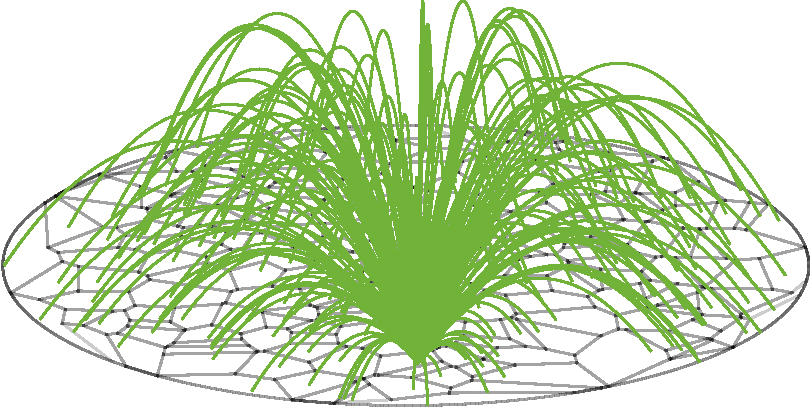
\includegraphics[width=0.4\textwidth]{gfx/chapter-monocentric/1.pdf}
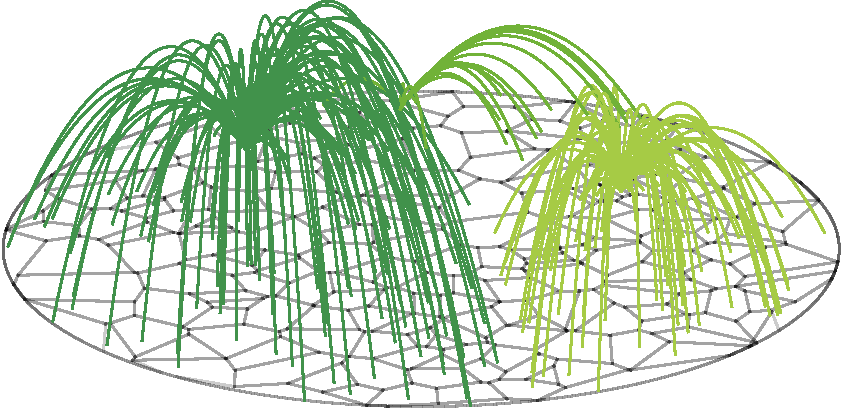
\includegraphics[width=0.4\textwidth]{gfx/chapter-monocentric/2.pdf}
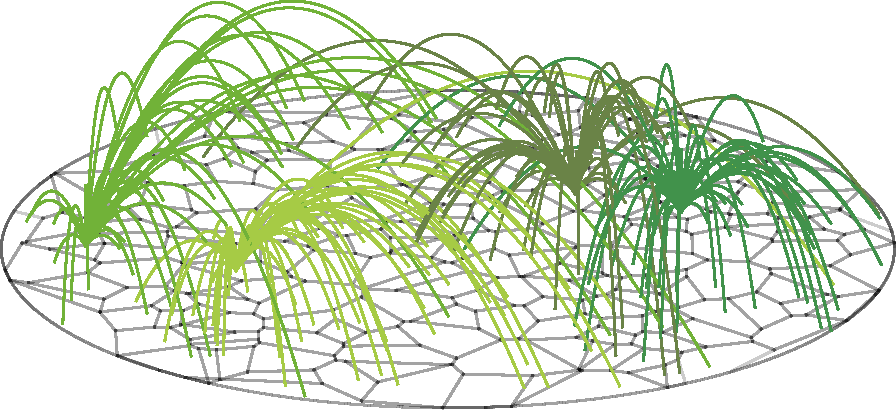
\includegraphics[width=0.4\textwidth]{gfx/chapter-monocentric/3.pdf}
\caption{The monocentric (top), distance-driven polycentric (middle)
  and attractivity-driven polycentric (bottom) regimes as produced by
  our model. Each link represents a commuting journey to an activity center. \label{fig:model_results}}
\end{figure}


From now on, we will assume that $\ell$ is large enough so that a
monocentric state exists for small values of the population. In this
regime, the value of $\eta$ prevails and the monocentric state evolves
to an attractivity-driven polycentric structure as the population
increases (if $\ell$ is too small, the monocentric regime does not
exist-see the Supplementary material~\cite{SM} for more details on
these points).  Starting from a small city with a monocentric
organisation, the traffic is negligible and $Z_{ij}\approx \eta_j$
which implies that all individual are going to choose the most
attractive center (with the largest value of $\eta_j$, say
$\eta_1$). When the number $P$ of households increases, the traffic
will also increase and some initially less attractive centers (with
smaller values of $\eta$) might become more attractive, leading to the
appearance of new subcenters characterized by a non-zero number of
commuters. More precisely, a new subcenter $j$ will appear when for an
individual $i$, we have $Z_{ij}>Z_{i1}$. The traffic so far is
$T(1)=P$ and $T(j)=0$ which leads to the equation
\begin{equation}
\eta_j-\frac{d_{ij}}{\ell}>\eta_1-\frac{d_{i1}}{\ell}\left[1+\left(\frac{P}{c}\right)^\mu\right]
\end{equation}
We assume that there are no spatial
correlations in the subcenter distribution, so that we can make the
approximation $d_{ij}\sim d_{i1}\sim L$. The new subcenter will thus
be such that $\eta_1-\eta_j$ is minimum implying that it will have the
second largest value denoted by $\eta_j=\eta_2$. For a uniform distribution
(details of the calculation can be found in the Supplementary
Material~\cite{SM}, section 2), on average
$\overline{\eta_1-\eta_2}\simeq 1/N_c$ leading to a critical value for
the population
%
\begin{equation}
P^*= c \left( \frac{\ell}{L N_c} \right)^{1/\mu}
\end{equation}
%
Whatever the system considered, there will therefore \emph{always} be
a critical value of the population above which the city becomes
polycentric (which can be smaller than one, in which case there is no
monocentric regime at all, see the Supplementary Material~\cite{SM}). The monocentric regime is therefore fundamentally
unstable with regards to population increase, which is in agreement with the fact that no major city in
the world exhibits a monocentric structure. We note that the smaller
the value of $\mu$ (or larger the value of the capacity $c$), the
larger the critical population value $P^*$ which means that cities
with a good road system capable of absorbing large traffic display a
monocentric structure for a longer period of time.


Having established that cities will eventually adopt a polycentric
structure, we can wonder how the number of subcenters varies with the
population. We compute the value of the population at which 
the $k^{th}$ center appears. We still assume that we are in the attractivity-driven regime and that, so far, $k-1$
centers have emerged with $\eta_{1} \geq \eta_{2} \geq \ldots \geq
\eta_{k-1}$~\cite{SM}, with a number of commuters $T(1), T(2), \ldots,
T(k-1)$, respectively. The next worker $i$ will choose the center $k$ if
\begin{equation}
Z_{ik} > \max_{j \in \left[1,k-1\right]} Z_{ij}
\end{equation}
which reads
\begin{equation}
\eta_k - \frac{d_{ik}}{\ell} > \max_{j \in \left[1,k-1\right]} \left\{
\eta_j - \frac{d_{ij}}{\ell} \left[ 1 + \left(
  \frac{T(j)}{c}\right)^\mu\right] \right\}
\end{equation}
The distribution of traffic $T(j)$ is narrow~\cite{SM}, which means that all the centers have roughly the same number of
commuters $T(j) \sim P/(k-1)$. As above we also assume that the
distance between the workers' households and the activity centers is
typically $d_{ij} \sim d_{ik} \sim L$. The previous expression now
reads
\begin{equation}
\frac{L}{\ell} \left( \frac{P}{(k-1)\,c} \right)^{\mu} > \max_{j \in
  \left[1,k-1\right]} \left( \eta_j \right) - \eta_k
\end{equation}
Following our definitions, $\max_{j \in \left[1,k-1\right]} \left(
\eta_j \right) = \eta_1$. According to order statistics, if the
$\eta_j$ are uniformly distributed, we have on average
$\overline{\eta_1 - \eta_k} = (k-1)/(N_c+1)$. It follows from these
assumptions that (1) the $k^{th}$ center to appear is the $k^{th}$ most attractive one (2) the average value of the population $\overline{P}_k$ at
which the $k^{th}$ center appears is given by:
%
\begin{equation}
\overline{P}_k = P^* \left( k-1 \right)^{\frac{\mu+1}{\mu}}
\label{eq:prediction}
\end{equation}
%
Conversely, the number $k$ of subcenters scales sublinearly with population as
\begin{equation}
k \sim \left( \frac{\overline{P}}{P^*} \right)^{\frac{\mu}{\mu + 1}}
\end{equation}
It is interesting to note that this result is robust: the dependence
is sublinear, \emph{whatever the distribution} of the random variable
$\eta$ (see the Supplementary Material~\cite{SM} for a discussion on this
point). We can therefore conclude that, probably very generally and
under mild assumptions, the number of activity subcenters in urban
areas scales sublinearly with their population where the prefactor and
the exponent depend on the properties of the transportation network of
the city under consideration. 

A previous study~\cite{Samaniego:2008} showed that the daily total
miles driven daily in a city --- the `total commuting
distance'---scales with the population as $L_{tot} \sim P^\gamma$
where $\gamma \in \left] 0.5, 1\right[$, which the authors interpreted
as cities having neither a neither totally centralized nor totally
decentralized structure. We can discuss this result within the
framework of our model in the following way. If the system was in the
pure attractivity-driven regime, we would have $L_{tot} \sim P$. But, if we
assume that we are in an intermediate regime where
Eq.~\ref{eq:prediction} holds, and where the system exhibits spatial
coherence~\cite{SM}, we can write the total length of commuting
journeys as
%
\begin{equation}
L_{tot} \sim P \frac{L}{\sqrt{k}}
\end{equation} 
%
Inverting the result from Eq.~\ref{eq:prediction} we therefore get
%
\begin{equation}
L_{tot} \sim P^{1-\frac{\beta}{2}}
\label{eq:beta}
\end{equation}
%
where $\beta = \frac{\mu}{\mu+1} \in \left[0 , 1\right]$. Our model is
thus consistent with the fact that the total traveled miles scales with
population with a non-trivial exponent comprised in $[0.5,1]$.\\


\begin{figure*}
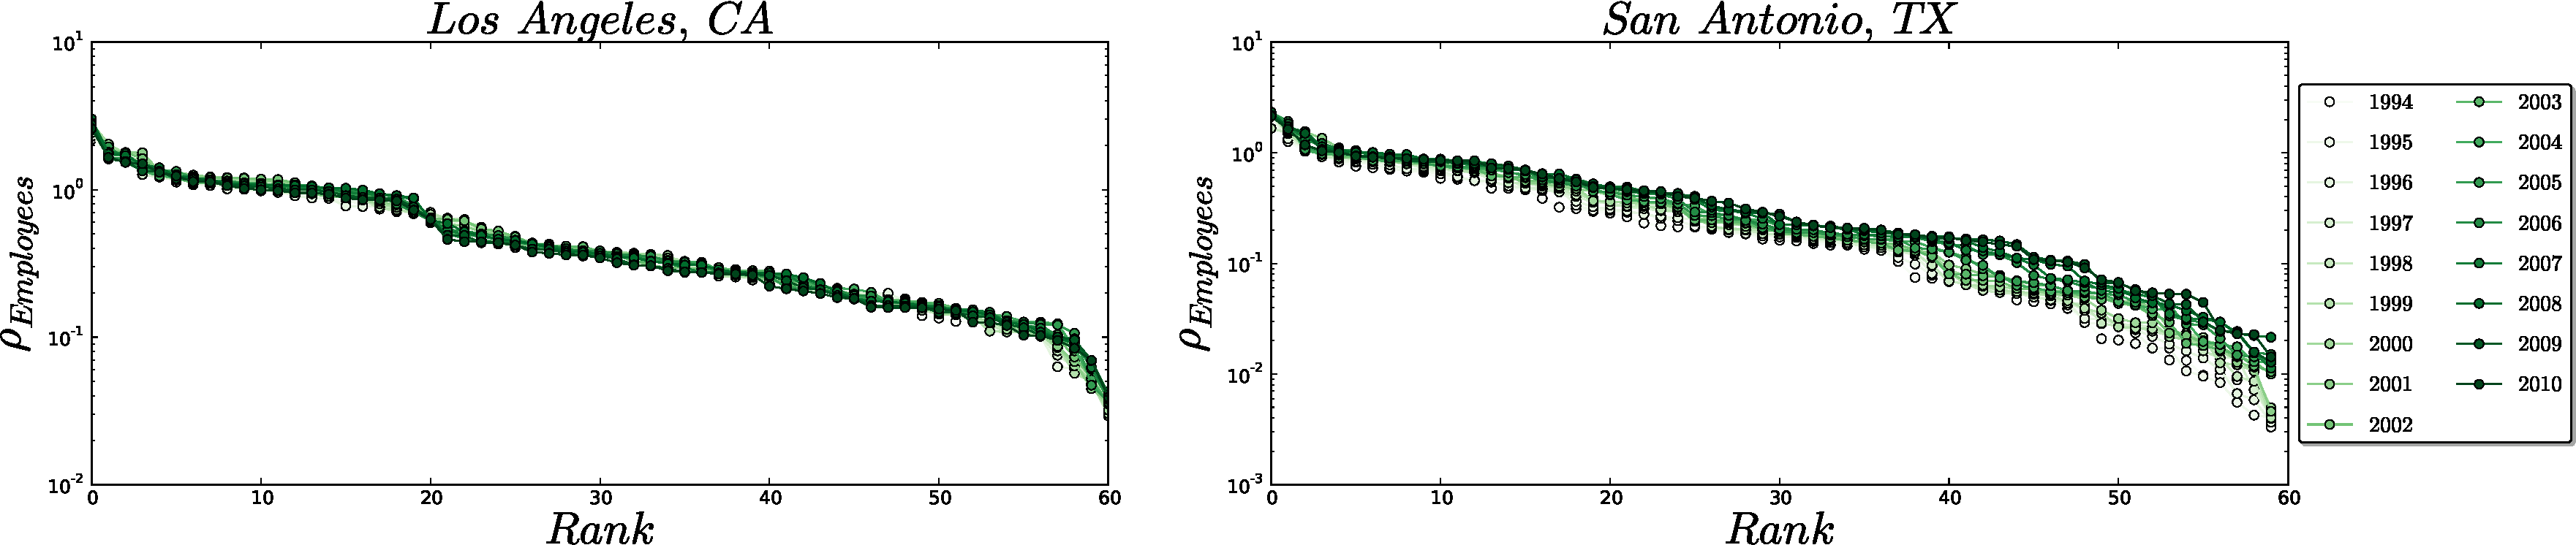
\includegraphics[width=\textwidth]{gfx/chapter-monocentric/4.pdf}
\caption{Rank-plot for the employment density (in employees per
  $km^2$) in Los Angeles, CA (left) and San Antonio, TX (right)
  between 1994 and 2010. See the Supplementary Material~\cite{SM} for more details. \label{fig:rank_plots}}
\end{figure*}

    \subsection{Empirical verification}
    \label{sub:empirical_verification}
    
People from the Census Bureau use the 2000 Census tract-to-tract commuting data
in order to get the employment density~\cite{Marlay:2010}. Use these data in
order to assess the employment density in 2000 MSAs. Use population data at the
same level in order to assess population density in 2000 MSAs.
Plot at several levels of the threshold and show the many different centers.
Propose a method to compute the number of centers (exponential, Loubar, etc.).\\
        \subsubsection{Counting the number of centers}
        \label{ssub:counting_the_number_of_centers}
        
        
We now test the prediction given by Eq. (\ref{eq:prediction}). For
that purpose, we collected data for the number of employees per Zip
Codes in the United States for 16 years, between 1994 and
2010~\cite{ZBPdata}, as well as the population of all cities in the US
between 1994 and 2010~\cite{CensusData}. We estimate the number of
subcenters by constructing the rank-plot of the employment density
$\rho$ (number of employees per $km^2$) for each Zip Code of a given
urban area~\cite{Griffith:1981,Dokmeci:1994}. These plots display a decay as fast as an exponential
(Fig.~\ref{fig:rank_plots}) which implies that there exists a natural
scale for the rank, that we interpret here as the typical number of
activity centers. It also implies that any reasonable method should
give an estimate of the number of subcenters of the same order of
magnitude (which would not be the case for slowly decaying function
such as power laws for example). We first note that for some cities
--typically large ones with stable populations
(Fig.~\ref{fig:rank_plots}, left)-- the employment spatial statistics
remained stable over the period of study. For other cities, we observe
large variation of the number of subcenters
(Fig.~\ref{fig:rank_plots}, right). We then plot (Fig.~\ref{fig:data})
the population $P$ of cities (with population $P>100$) versus the
estimated number of subcenters $k$ (the dispersion in the scatterplot
probably results from the fact that different cities have different
resilience levels to congestion). On average, we observe a power law
dependance with exponent $\delta=1.56 \pm 0.15$ (the result is robust
with regards to the estimate of $k$, see the Supplementary
Material~\cite{SM} for more details). Inverting this relation gives us
the number of subcenters as a function of the population
%
\begin{equation}
k \sim P^{\beta}
\end{equation}
%
with $\beta \sim 0.64$. This result is strikingly in agreement with
the prediction given by our model: the number of subcenters in a city
scales sublinearly with its population.\\

\begin{figure}
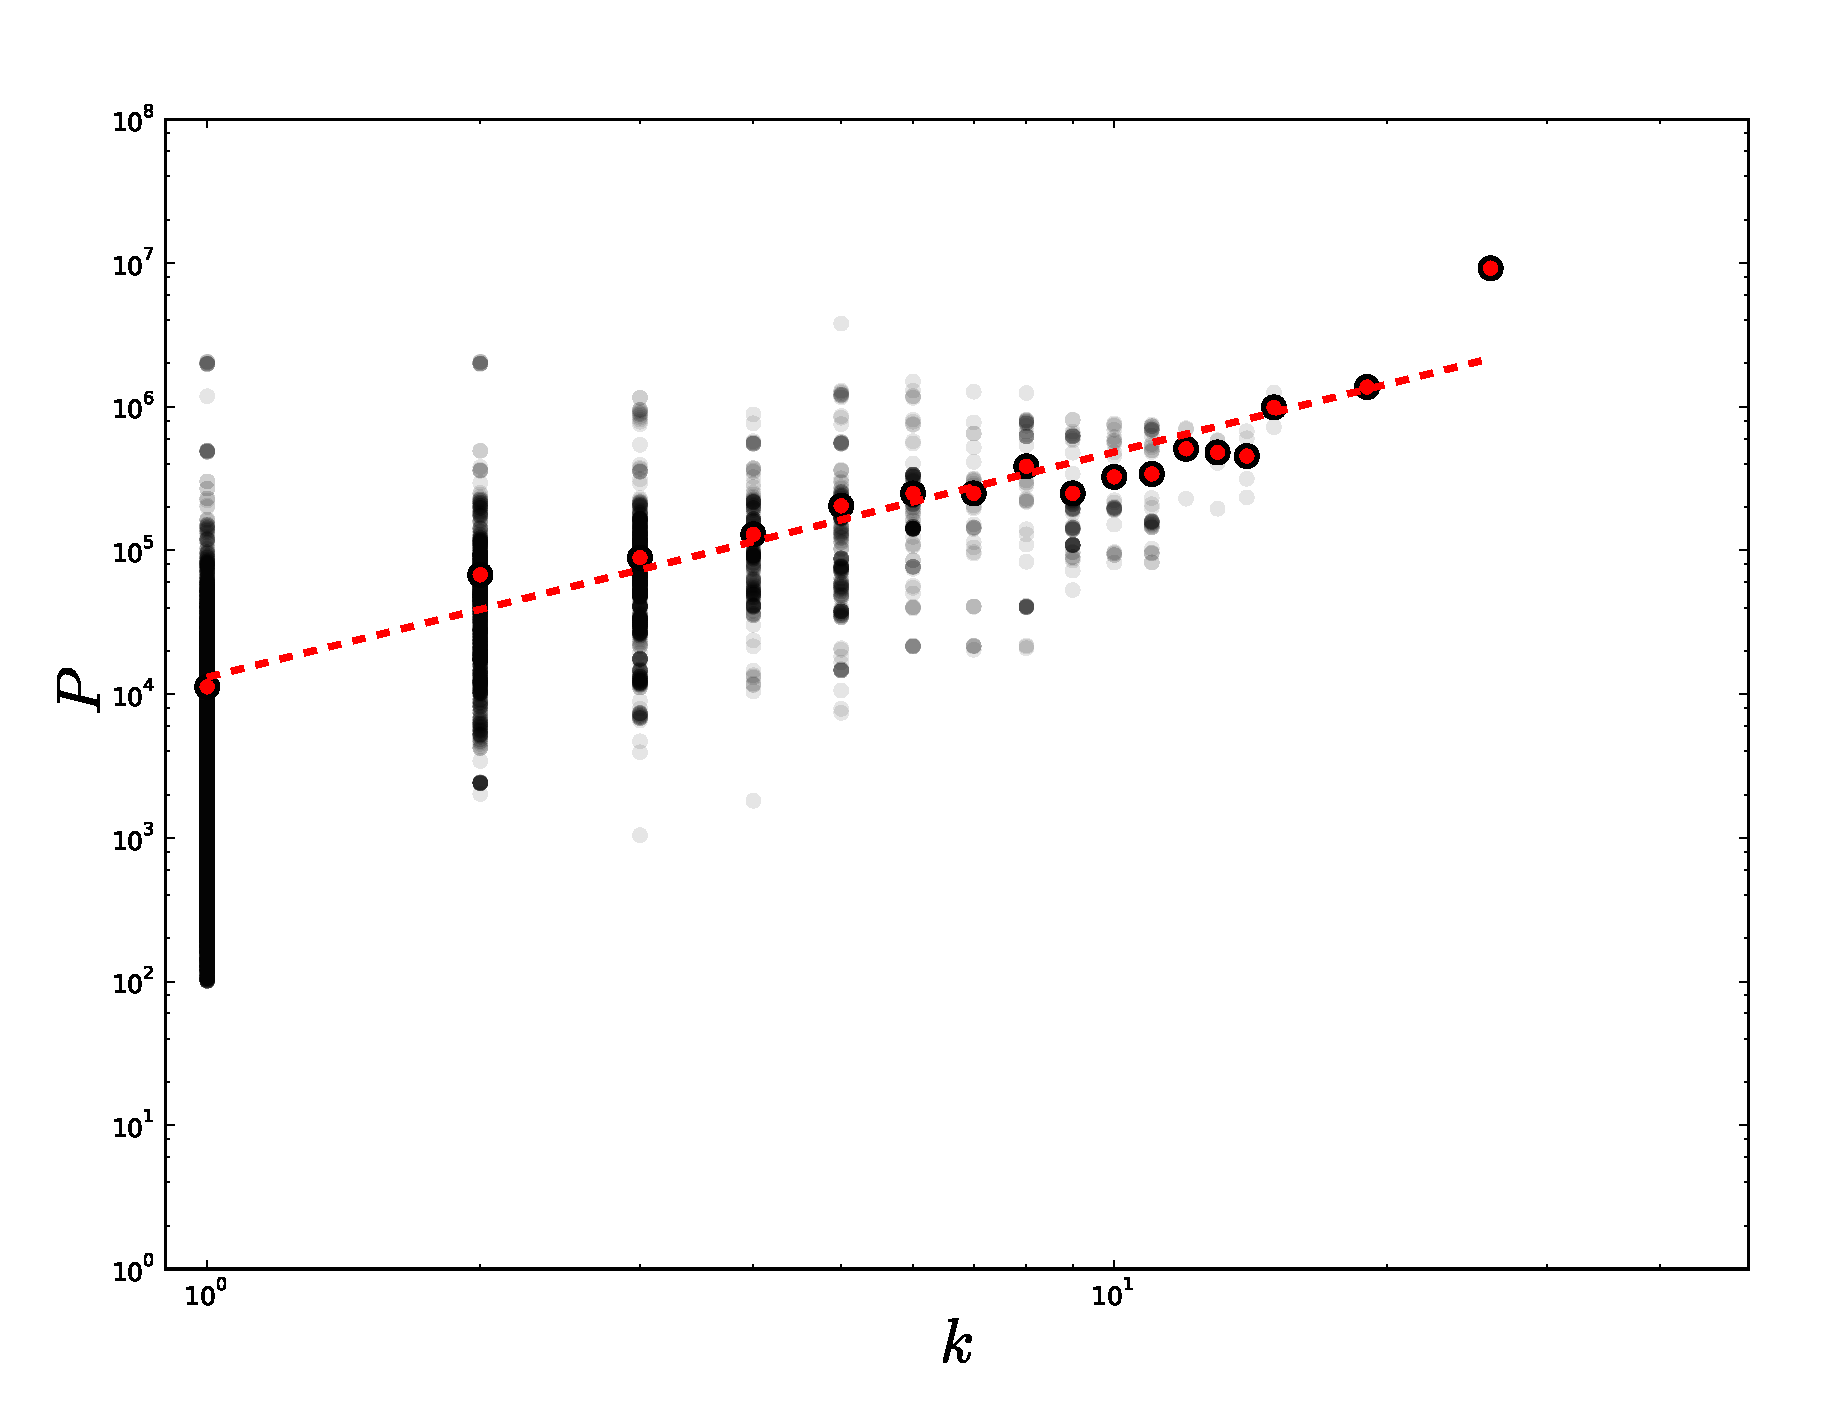
\includegraphics[width=0.5\textwidth]{gfx/chapter-monocentric/5.pdf}
\caption{Scatter plot of the estimated number of subcenters versus the
  population for about 9000 cities with population over 100 people in
  the U.S. The red dots represent the average population for a given
  number of subcenters. We fit this average with a power-law
  dependence (represented by a red dashed line) giving an exponent
  $\delta=1.56\pm 0.15$ ($r^2=0.87$). See the Supplementary Material~\cite{SM} for more details on the computation of $k$ and the robustness of the results. \label{fig:data}}
\end{figure}

Using the measured value of $\beta$ and Eq. (\ref{eq:beta}) we can estimate the exponent of
the scaling of $L_{tot}$ with the population and find $L_{tot} \sim
P^{\,0.68}$ which agrees very well with the value $0.66$ measured
in~\cite{Samaniego:2008} directly on the data of the daily total miles
driven in more than $400$ cities in the US.\\

While agglomeration economies seem to be the basic process explaining
the existence of cities and their spectacular resilience, this study
brings evidence that congestion is the driving force that tears them
apart. The non trivial spatial patterns observed in large cities can
thus be understood as a result of the interplay between these
competing processes. We believe that the present model represents an
important step towards a quantitative, predictive science of
cities. More generally, this microscopic approach is an interesting
example of an out-of-equilibrium model: it is governed by local
optimization with saturation effects, leads to different regimes, and
is characterized by non-trivial dynamical exponents. In this respect,
we believe that this discrete approach might be of use in the study of
pattern formation in biology --which have been so far explored from a
global optimisation perspective~\cite{Ashton:2005} or using
coarse-grained reaction-diffusion approaches with density dependent
diffusion coefficients~\cite{Cates:2012}-- to compute quantities that
are out of reach within the current methods.

\section{Proviso}
\label{sec:proviso}

All methods to measure the number of centers do not consider the spatial
contiguity of different areal units. It might be that we find different areal
nits that are in fact part of the same center [Show example]. So all these
methods do not output a `real' number of centers, but rather provide values that
are coherent across urban areas and allow their comparison.
